\documentclass[memoire.tex]{subfiles}

\chapter{Analyse des solutions logicielles existantes}

Maintenant que nous avons vu les différentes architecture Big Data existantes et que nous les avons décomposés, on va s'intéresser plus en détail à chaque composant de ces architecture. Pour chaque composant, nous allons présenter diverses solutions existantes permettant de remplir le rôle de ce dernier. Pour chacune de ses solutions, nous allons voir leurs avantages et inconvénients et leurs manière de fonctionner dans le but de pouvoir en dégager des critères de sélections.

\section{Message Broker}

Un Message broker~\cite{MSG_BROKER}, Agent de message en français, est un moyen de communication utilisant des messages entre deux applications (Ex: Communication entre un serveur et un client). Un message broker permet une communication asynchrone entre applications. L'utilisation de cette solution permet de pouvoir facilement filtrer les messages que l'on reçoit et de stocker temporairement les messages reçus afin d'éviter les pertes de données. Ce dernier cas, s'avère très utile dans le cas où l'application chargée de la réception des données n'est pas en fonctionnement pendant un certains temps. Il existe deux types de communications avec un message broker : 

\subsubsection*{Publisher / Subscriber}

Dans ce mécanisme, l'entité envoyant les données est nommé "Publisher" et l'entité les récupérant est nommé "Subscriber". Le publisher va envoyer des données dans des topics \footnote{Un topic est une catégorie dans laquelle les messages produit sont stockés.} afin que les Subscribers de ce topic puissent les récupérer. Un publisher peut envoyer des données dans un ou plusieurs topics, et les subscribers peuvent être abonné à un ou plusieurs topics (Voir figure 2.1). 


\begin{figure}[!h]
	\centering 
	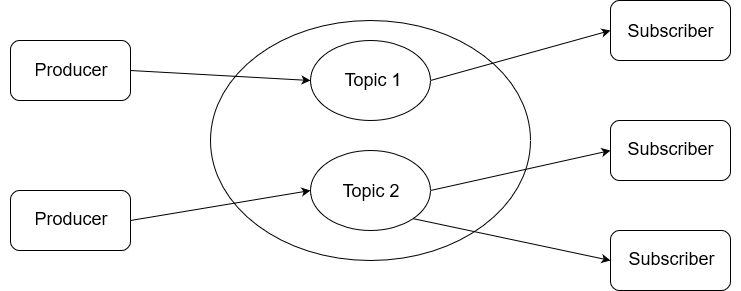
\includegraphics[scale=0.50]{img/producer_subscriber.png}
	\caption{Schéma du principe Publisher(Producer)/Subscriber}
	\label{Lambda}
\end{figure}

\subsubsection*{Point-to-point communication}

La communication point à point est la forme la plus simple de Producteur/Consommateur. Le producteur envoie ses données dans une queue et le consommateur va lire les messages dans la queue. Tout comme le modèle précédent, il peut y avoir plusieurs producteur et consommateurs sur la même queue, mais si plusieurs consommateurs sont présents, ils ne recevront des portions différentes des messages afin de favoriser le traitement concurrentiel.

\subsection{Kafka}

Apache Kafka~\cite{KAFKA}\cite{KAFKA2} est un système de messages distribué, développé par Linkedin.

Kafka utilise le système communication du Publisher(Producer) / Subscriber en utilisant un élément unique, appelé broker. Afin de faciliter la mise à l'échelle et le partitionnement des données, il est possible d'instancier autant que broker que l'on souhaite afin d'augmenter le débit et la résilience du produit.

Une autre brique est utilise par Kafka afin de gérer l'état des différents brokers, il s'agit de Apache ZooKeeper. Il permet de stocker facilement toutes les méta-données de chaque broker, comme par exemple le nombre de données injectées dans chaque topics, ou bien la répartition des différentes topics sur chaque broker (Voir figure {\ref{cluster-kafka}}.

\begin{figure}[hbt!]
	\centering 
	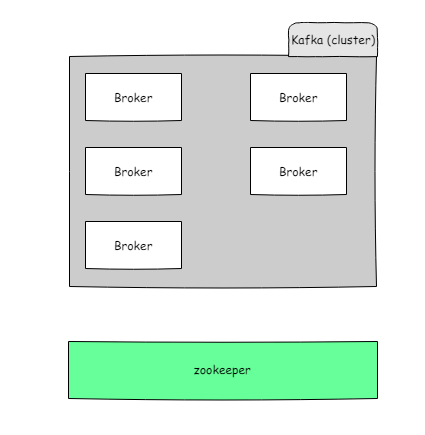
\includegraphics[scale=0.50]{img/kafka_broker.png}
	\caption{Schéma d'un cluster Kafka et des ces composants}
	\label{cluster-kafka}
\end{figure}

Les messages envoyés à Kafka sont stockés sur disque dans le format appelé \textbf{LOG}.
Ce format n'a rien à voir avec les logs applicatifs, il s’agit d’un tableau de messages ordonnés. L'ordonnancement est réalisé à partir de la date d'arrivée du message. Chaque message se voit donner un index aussi appelé offset.

\subsection{ActiveMQ}

Comme Kafka, ActiveMQ utilise le système de communication Publisher(Producer) / Subscriber. L'intérêt principal d'ActiveMQ est de connecter différentes application réaliser avec des langages différents avec l'aide des API fournit.

De la même manière que Kafka, il permet de se mettre à l'échelle très facilement mais il n'utilise pas de brique intermédiaire afin de gérer les états des brokers (ZooKeeper). Les différentes instances d'ActiveMQ utilisent un système de multicast afin de se découvrir.

\subsection{RabbitMQ}

Contrairement à Kafka et ActiveMQ, RabbitMQ utilise le système de communication Point-to-Point. Cela permet de garantir qu'un seul consommateur vas être en mesure de lire le message présent dans la queue.

RabbitMQ n'utilise pas de brique extérieure afin de gérer la mise à l'échelle, mais il suit le même mode de fonctionnement que ces deux concurrents, c'est à dire un système de partition.

\subsection*{Conclusion}

Nous pouvons constater que ces trois solutions se ressemblent, elle se se départagent uniquement sur quelques points. L'utilisation de différents protocoles, le mécanisme de communication ou bien la manière de se mettre à l'échelle. 

\section{Ingestion/Extraction de données}

La première catégorie, qui est aussi la première étape d'une architecture Big Data, c'est le récupération de données. Plus précisément comment nous allons récupérer des données, soit via des requêtes sur des sources externes, soit des sources externes nous envoie directement des données. 

Il existe deux approches afin d'effectuer cette tâche, soit l'utilisation d'un logiciel appelé ETL ou ELT ou bien, l'écriture de programme. Un logiciel ETL (Extract Transform \& Load) ou ELT (Extract Load \& Transform), sont des solutions permettant d'extraire des données depuis des sources, appliquer une transformation sur ces données et enfin les charger dans une solution de stockage. En plus d'être solution complète, la gestion du flux des données est entièrement paramétrable à l'aide d'une interface graphique afin de faciliter l'utilisation de ces outils. La distinction entre ETL et ELT est l'ordre dans lequel les opérations sont effectués, soit les données sont d'abord transformés puis stockés (ETL) soit l'inverse (ELT). 
Les deux premières solutions que nous allons aborder pour répondre à la problématique de l'ingestion des données sont des ETL/ELT.

\subsection{Apache Nifi}

\subsection{Talend}

\subsection{Solution maison}

Il est aussi tout à fait possible d'envisager d'écrire un programme simple permettant d'extraire des données des données depuis une source pour ensuite les injecter dans une base et lancer le traitement des données. Pour nous aider dans cette tâche, il existe dans une majorité des langages des connecteurs permettent d'interagir par exemple avec des bases de données. Toutefois, il est important de respecter certains critères avant de se lancer dans le développement d'un programme maison. Comme on l'a vu tout au long de notre recherche, l'un des points clés du Big Data est sa capacité de mise à l'échelle. Il faut donc choisir le langage et/ou un framework pouvant lui aussi être mis à l'échelle facilement, c'est à dire qu'il doit adopté une architecture réactive ({\ref{a:architecture-reactive}}). Deux frameworks très connu utilisant cette architecture sont Akka et Vert.x. Akka utilise le principe de concurrence Acteur tandis que Vert.x utilise le principe d'évènements. Akka supporte officiellement Java et Scala et on peut facilement l'utiliser avec d'autres langages de la JVM\footnote{Machine virtuelle java}. De son côté, Vert.x supporte de manière officielle Java, Scala, Kotlin, Javascript, Ruby et Ceylon. Il existe des modules pour Vert.x permettant de supporter d'autres langages comme le python par exemple mais il ne sont pas maintenu par Vert.x.

\subsection*{Conclusion}

Pour conclure sur cette partie, nous avons donc le choix d'utiliser des solutions complètes configurable facilement, ou bien écrire nous même un programme réalisant l'ingestion des données. L'utilisation d'une solution complète peut paraître la plus attractive mais elle est plus consommatrice en ressources qu'un simple en programme.

\section{Traitement des données}

Après avoir récupérer des données, nous devons passer à l'étape du traitements des données. Celui ci à plusieurs rôles, en effet il peut servir à formater les données, leurs apportés de la cohérence en les combinant à des données déjà présentent. Et pour finir les rediriger vers le stockage souhaité. Le traitement des données peut se faire de deux manière différentes. La première solution est le traitement par Batch, et la seconde est le traitement en temps réel~\cite{TYPE_TRAITEMENT_DONNEES}\cite{TYPE_TRAITEMENT_DONNEES2}. Chacune possède ses avantages et inconvénients, nous allons voir ça plus en détails.

\subsection{Batch}

Le traitement par Batch (Traitement par lot), consiste à traiter un important volume de données à un instant T. Le traitement par batch est surtout utilisé dans les cas ou nous avons des données stockés de manière journalière, et que nous avons besoin de tout traités en fin de journée. Il n'est pas rare de voir des tâches de traitements par Batch s'exécuter dans la nuit, étant donnée que l'on traite une masse de donnée importante, on sollicite la machine pendant une longue période. Réaliser ce traitement durant des périodes creuses, permet de largement diminuer l'impact sur l'utilisation de la plateforme (\ref{traitement-batch}).

\begin{figure}[!h]
	\centering 
	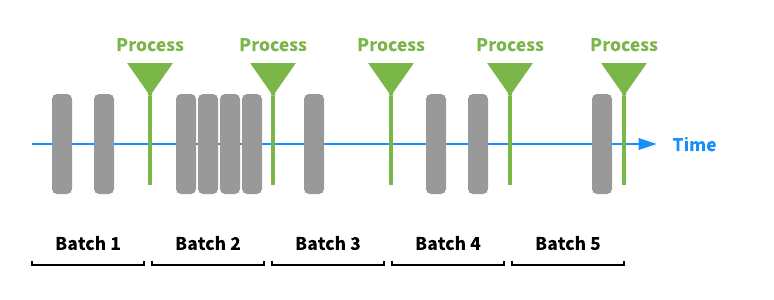
\includegraphics[scale=0.50]{img/batch-processing.png}
	\caption{Schéma du traitement par batch}
	\label{traitement-batch}
\end{figure}

Nous allons nous pencher sur les solutions existantes, implémentant un traitement par batch.

\subsubsection{Apache Spark}

Spark est un moteur de traitement de données distribué, il répond à de nombreux cas d'utilisation. En plus du moteur de traitement de données, Spark possède des librairies SQL, d'apprentissage automatique, de calcul des graphes ainsi que le traitement de flux qui sera abordé dans la partie {\ref{spark-streaming}} sur Spark Streaming. Spark supporte différents langages de programmation, Java, Scala, Python et R. 

Spark à des performances accrue car entre chaque étape des calculs, au lieu de stocker les résultats sur disque il les garde en RAM.

\subsubsection{Hadoop MapReduce}

MapReduce est aussi un moteur de traitement de données distribué, mais il répond à de moins nombreux cas d'utilisation que son concurrent Spark. Il ne possède qu'une seule librairie permettant de faire de l'apprentissage automatique. Il manque donc de librairies  SQL, de calcul des graphes ainsi que de traitement de flux contrairement à son concurrent.

Au niveau des performances, MapReduce se montre moins efficace que Spark. Là où Spark va stocker en RAM tout les résultats intermédiaire, MapReduce va stocker ces résultats sur disque. Cela a un impact non négligeable sur les performances, mais il permet aussi de diminuer les coûts de la plateforme et de garantir une meilleure tolérance à la panne.

\subsubsection*{Conclusion}

Ces deux solutions sont intéressantes, mais couvre des cas d'utilisation vraiment différents. Il est donc très important de bien cibler son besoin afin de faire le bon choix pour son architecture.

\subsection{Streaming}

Un traitement de données est considéré comme étant en temps réel si il s'effectue en une seconde ou moins après la réception de la donnée. Il peut être de deux types, soit des micro batchs soit en streaming.

\subsubsection*{Micro-Batch}

Le traitement par micro batch est basé sur le même principe que le traitement par batch, à l'exception qu'il s'exécute beaucoup plus régulièrement (Toutes les secondes ou moins) et que le nombre de données à traiter est donc significativement plus faible. Le micro batch est surtout utilisé dans les cas où notre système ne peut pas directement réagir lorsqu'une donnée arrive, on va donc récupérer les données très régulièrement afin de garantir un traitement en temps réel ou du moins dans le délai le plus bref possible.

\subsubsection*{Streaming}

Le traitement en streaming (Traitement de flux), s'appuie sur l'architecture réactive ({\ref{a:architecture-reactive}}). En effet, contrairement aux traitements par batch et micro batch, ici on ne vas pas récupérer des données de temps en temps. Dès qu'une donnée arrive on va la récupérer et la traiter immédiatement. De par son fonctionnement, le traitement en streaming ne nécessite pas de stockage en amont contrairement aux autres type de traitement (\ref{traitement-streaming}).

\begin{figure}[!h]
	\centering 
	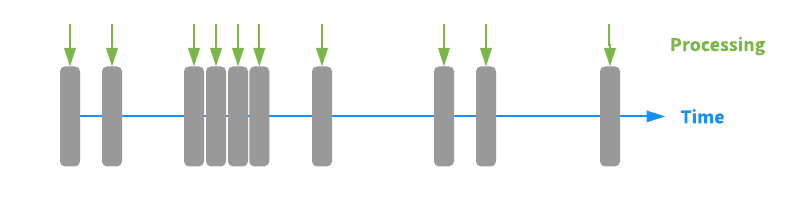
\includegraphics[scale=0.50]{img/stream-processing.png}
	\caption{Schéma du traitement en streaming}
	\label{traitement-streaming}
\end{figure}

Nous allons maintenant nous intéresser aux différentes solutions proposant ce type de traitement.

\subsubsection{Apache Spark Streaming}
\label{spark-streaming}

Spark Streaming est comme on l'a vu précédemment une version de Spark étudié pour le traitement en temps réel. Il bénéficie donc du large choix de librairie de Spark. 

Spark Streaming à une latence assez faible mais pas suffisamment pour s'orienter vers du traitement en streaming il est plus orienté pour un traitement en micro-batch.

Spark Streaming s'avère très utile dans le cadre d'une architecture Lambda, comme on l'a vue dans cette architecture les traitements en batch et en temps réel sont effectués par des outils différents. Spark Streaming permet d'avoir la même base de code pour le traitement en bacth et en temps réel, cela permet d'éviter de la duplication de code et de pouvoir n'utiliser entre autre qu'un seul outil pour le traitement des données..

\subsubsection{Apache Storm}

Apache Storm propose une sélection moins importante de langage de programmation que Spark Streaming. Il ne propose que le Java, Scala et Clojure.

Contrairement à Spark Streaming, Apache Storm possède une latence beaucoup plus faible ce qui lui permet de gérer le traitement en streaming sans aucun problème.

Tout comme Spark Streaming, Apache Storm stock les résultats intermédiaires en RAM pour garantir des performances accrues.

Apache Storm ne propose pas de librairie de calcul des graphes et n'a pas de librairie d'apprentissage automatique intégré, il faudra en installer une compatible contrairement à Spark Streaming.

Apache Storm à l'opposé de son concurrent ne permet pas de garder la même base de code entre le traitement en batch et en streaming, son utilisation se place par conséquent plus dans le cadre d'une architecture Kappa.

\subsubsection*{Conclusion}

Malgré un mode de fonctionnement similaire, ces deux solutions peuvent se démarquer sur des points important qui nous permettra de définir des critères précis par rapport à leur utilisation.


\section{Stockage des données}

Une partie très importante du Big Data est le stockage des nombreuses données que l'ont reçoit. Il existe énormément de manières différentes de stocker des données selon la manière dont nous voulons les utiliser par la suite et surtout selon leurs format. De plus l'utilisation de plusieurs bases de données est très courante, généralement une base de données est utilisée pour le stockage des données brutes avant leur traitements (appelé lac de données) puis une autre base de données correspondant au nouveau format des données est utilisé pour améliorer les performances. Le stockage des données dans le Big Data doit s'assurer de pouvoir stocker toutes les données reçu et avoir une très haute disponibilité. Pour cela de la réplication de données et une mise à l'échelle pour la lecture et l'écriture des données. Cela implique de s'éloigner des bases de données relationnelle et de s'orienter vers des solutions NoSQL qui facilite la mise en place de ces concept. Nous n'allons pas voir en détail le fonctionnement des bases de données NoSQL, nous nous contenterons de voir si les bases de données intègrent bien ces concepts et si elles ont des particularités sur la manière de traiter les données. Si vous souhaitez voir plus en détail le fonctionnement des bases de données NoSQL je vous conseille de lire l'article de Sonia Guehis et Marta Rukoz à ce sujet~\cite{}.

\subsection{Base de données de séries temporelles}

La première catégorie de base de données que nous allons traiter, est la base de données de séries temporelles. Ce type de stockage est de plus en plus important avec l'explosion de l'IoT qui est un des domaine générant le plus de donnée de séries temporelles.

Une série temporelle est tout simplement une valeur daté, par exemple la température d'un processeur à un instant T.

\subsubsection{OpenTSDB}

OpenTSDB est une base de données Open Source sous la licence GPL3 écrit en Java.

Afin de stocker les données, OpenTSDB se base sur une autre base de données appelé HBase, nous verrons plus en détail HBase dans la partie {\ref{hbase}}. Cette solution implique donc que vous avez déjà HBase d'installer et d'avoir les connaissances nécessaire pour le configurer correctement afin de garantir des bon débit de lecture et d'écriture.

OpenTSDB ne fournit pas d'outil de requêtage simplifié, il faut donc être familier avec HBase pour récupérer des données stockées dans OpenTSDB.

\subsubsection{InfluxDB}

InfluxDB est une solution Open Source développé par InfluxData sous la licence MIT et écrit en Go.

Contrairement à OpenTSDB, InfluxDB n'utilise de solution externe pour le stockage des données. Ils possède sa propre solution optimisé pour les données de série temporelle. Cela à un double avantage. Premièrement, pas besoin d'installer une autre base de données et d'avoir les connaissances nécessaire pour la configurer pour des données de série temporelles. Cela permet aussi d'avoir des performances accrues, l'architecture de stockage étant crée dans le seul but de stocker des données de série temporelle, il est normal que les performances soient meilleures que pour une solution qui peut gérer plusieurs formats de données.

Par rapport à son concurrent, InfluxDB propose une solution de requetâge de données simplifiant en utilisant le langage SQL.

\subsubsection*{Conclusion}

Nous pouvons constater que InfluxDB à l'air d'être la meilleure solution pour le stockage de série temporelle, mais le fait que OpenTSDB utilise HBase peut être un critère de choix pour certaines personnes pour le choix de leur architecture.

\subsection{Base de données orientée graphe}

Les bases de données orientée graphe sont apparu afin de permettre de stocker facilement les relations présente entre plusieurs données. Une base de donnée de graph est basé sur les bases de données orienté objet mais avec l'utilisation de la théorie des graphes. Le stockage des données est constitué de nœuds qui représentent les données et d'arcs qui sont des pointeurs physique représentant les relations entre chaque nœuds. Ce type de bases de données s'avère très utile dans le cadre des études des relations entre de nombreuses de données, ce qui souvent le cas dans le domaine du Big Data. La figure {\ref{graph-exemple}} montre un exemple de graphe qui peut être stocké dans une base de données orientée graph.

\begin{figure}[!h]
	\centering 
	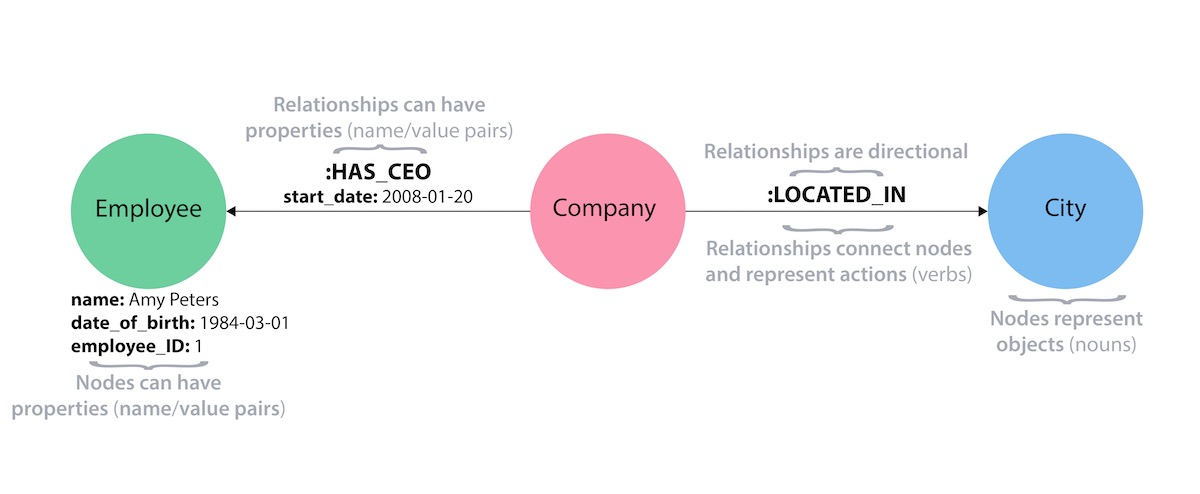
\includegraphics[scale=0.35]{img/graph_exemple.jpg}
	\captionsource{Exemple d'un graphe dans une base de données orientée graphe}{https://neo4j.com/developer/graph-database/}
	\label{graph-exemple}
\end{figure}

\subsubsection{Neo4j}

Neo4J est une base de données orientée graphe native écrite en Java et créer par l'entreprise portant le même nom. Il existe deux version de Neo4J, une version communautaire qui est open source sous la licence GPL3 et une version entreprise qui elle n'est pas open source. La solution communautaire manque de module de sécurité et ne propose de solution de mise à l'échelle.

Neo4J propose une longue liste de langage compatible, .Net, Clojure, Elixir, Go, Groovy, Haskell, Java, JavaScript, Perl, PHP, Python, Ruby et Scala.

Un atout de Neo4J est que c'est une solution native, cela permet une installation rapide et aucune dépendance nécessaire. Neo4J propose une interface web intégré pour la visualisation des graphes ainsi que pour l"écriture de requête avec leur propre langage nommé Cypher. Voici un exemple de requête utilisant le langage Cypher :

\begin{verbatim}
(p:Person {name: "Jennifer"})-[rel:LIKES]->(g:Technology {type: "Graphs"})
\end{verbatim}

Cette requête permet de récupérer la relation qui représente le fait que Jennifer aime la technologie.

Neo4J propose une mise à l'échelle pour la lecture ce qui la rend très rapide, malheureusement l'écriture n'est pas mise à l'échelle. Les performances en écriture restent très performantes mais l'insertion d'énormément de données sur une longue période de temps peut s'avérer assez lente.

\subsubsection{JanusGraph}

JanusGraph est une solution open source sous la licence Apache 2 écrit en Java.

Contrairement à Neo4J, la liste de langage supportés par Janusgraph est beaucoup moins importante. Il ne supporte que le Java, Python et Clojure.

JanusGraph n'est pas une solution native, il s'appuie sur Hbase (voir partie {\ref{hbase}}) ou Cassandra (voir partie {\ref{cassandra}}) pour le stockage des données et pour l'indexation il est fortement recommandé d'utiliser ElasticSearch (voir partie {\ref{elasticsearch}}) ou Solr (voir partie {\ref{solr}}) qui sont des moteurs d'indexation. Cela implique donc qu'il est nécessaire d'avoir à disposition ces solutions et de les maitriser afin de permettre leurs communication.

JanusGraph ne possède pas d'interface web, mais comme il s'appuie sur une solution de requêtage open source, cela lui permet de bénéficier d'interface web déjà développées. L'interface web la plus intéressante est Linkurious. 

Le langage de requêtage utilisé par JanusGraph est Gremlin, il est aussi facile à utiliser que Cypher mais les requête ne sont pas formées de la même manière. Voici un exemple de requête avec le langage Gremlin : 

\begin{verbatim}
g.V().has('name', 'hercules').out('father').out('father').values('name')
\end{verbatim}

Cette requête permet de récupérer le nom du grand père du nœud ayant comme nom hercules.

JanusGraph propose lui aussi une mise à l'échelle pour la lecture des données et avec des performances similaire à son concurrent. Mais il ne s'arrête pas là, grâce à son utilisation de brique extérieures (HBase ou Cassandra), il propose aussi une mise à l'échelle pour l'écriture des données. 

\subsubsection*{Conclusion}

Nous pouvons constater que sur les deux solutions que nous avons étudier, la différence majeure réside sur le fait que Neo4J est une solution native tandis que JanusGraph s'appuie sur des technologies déjà existante.

\subsection{Base de données clés/valeurs}

Les bases de données clés / valeurs se repose sur une structure très simple, qui est probablement la structure de données la plus simple. Le principe repose sur le fait qu'on ne peut y stocker uniquement des paires de clés et de valeurs. La récupération des valeurs s'effectue via une clé connue. Ce système de stockage ressemble au HashMap que l'on peut utiliser dans différents langages. Au delà de ce principe de paires, il n'y aucune structure des données, cela permet de pouvoir stocker n'importe quelle donnée sans avoir à définir un schéma à respecter et donc de réduire l'espace nécessaire.

Ce système de stockage étant trop simple pour répondre aux besoins d'application complexes trouvent néanmoins son intérêt dans la cadre de système embarqués ou bien si il y a un besoin de traitement de données à très haute performance.

\subsubsection{Redis}

Redis est développé par Redis Lab et écrit en C, il est open source sous la licence BSD.

Redis propose un support d'un très grand nombre de langage de programmation, il en propose plus de 20 dont par exemple Java, Python, C++ et Go.

Redis opère principalement sur la mémoire RAM pour garantir la vitesse la plus élevée possible. Il propose tout de même une solution de "persistance" via des snapshots effectué régulièrement. Les snapshots sont des sauvegarde de ce qui est stocké sur la RAM à un instant T.

Redis propose également un cluster, permettant de répartir la charge sur différents nœuds. ainsi qu'une réplication des données.


\subsubsection{RocksDB}

RocksDB est une solution open source sous les licences GPLv2 et Apache 2, il est écrit en C++ et développé par Facebook.

Contrairement à Redis, RocksDB supporte beaucoup moins de langage, il ne propose le support que pour Java et C++.

A l'opposé de Redis, RocksDB opère principalement sur disque, ce qui permet de rendre les données persistante à tout moment et de pouvoir interagir avec des données plus volumineuses. Afin de palier le manque de vitesse par rapport à son concurent qui utilise la RAM, RocksDB profite du stockage flash apporté par les nouveaux SSD proposant des débits de plus en plus rapide.

Tandis que Redis est une solution accessible par différente applications sur le réseau, RocksDB lui est une solution embarqué sur un appareil, il est accessible uniquement sur la machine sur laquelle il est installé. Cela limite donc les possibilités de mise à l'échelle mais permet de réduire les interactions sur le stockage.

\subsubsection*{Conclusion}

Nous pouvons constater que ces deux solutions de stockage basé sur le modèle clé/valeur sont complètement opposé. Cela va nous permettre de facilement dégager des critères pour définir les situations correspondants le mieux à chacun de ces outils.

\subsection{Moteur d'indexation}

les moteurs d'indexation sont une catégorie de bases de données qui en général ne servent de stockage permanent, mais d'outil intermédiaire pour la visualisation et l'analyse des données. Le principe de cet solution est d'indexer toutes les données afin de permettre des requêtes beaucoup plus rapide, spécialement pour des opérations de recherche. Il est en effet beaucoup plus rapide de rechercher une donnée par avec un catalogue qu'en parcourant toutes les données stockées. Cela permet de faire des recherches plus avancées sur les données tout en pouvant facilement mettre à l'échelle l'exécution des recherches et le stockage des données. Afin de stocker des données dans ce genre de base de données, il suffit de créer un index pour un jeu de données en définissant le type de nos champs. Une fois cela fait, au moment d'injection des données dans la base de données, il suffit de spécifier l'index à utiliser. Ensuite les données seront indexées en fonction des paramètres présent dans l'index, cette opération peut prendre un peu de temps, mais une fois effectué, les recherches seront très rapide.

\subsubsection{Elasticsearch}
\label{elasticsearch}

Elasticsearch est une solution open source sous la licence Apache 2 écrit en Java par l'entreprise Elastic.

Le moteur de recherche utilisé par Elasticsearch est Apache Lucene.

Elasticsearch est une solution native, c'est à dire qu'il ne nécessite aucune installation de dépendances et que tous ses composants ont été conçus dans le but de créer un moteur d'indexation. Elasticsearch possède un mécanisme de mise à l'échelle. De par son indexation "strict", Elasticsearch permet un traitement de données structurés en temps réel. Il propose aussi une intégration de module d'apprentissage automatique permettant la détection d'anomalies en temps réel.

Elasticsearch fait parti de la suite elastic qui propose aussi un outil d'analyse et de visualisation des données nommé Kibana (Voir partie {\ref{kibana}}). Kibana et Elasticsearch sont entièrement compatible, plus précisément Kibana s'intègre uniquement avec Elasticsearch.

\subsubsection{Apache Solr}
\label{solr}

Apache Solr est une solution open source sous la licence Apache 2 écrit en Java par l'entreprise Apache.

Solr est très similaire à Elasticsearch en terme de performances malgré une architecture vraiment différente. En effet, Solr s'appuie sur plusieurs dépendances afin de proposer une solution complète contrairement à Elasticsearch qui lui ne nécessite aucune brique extérieure. Le seul point commun avec Elasticsearch est que Solr aussi utilise Apache Lucene. Pour le stockage des données l'utilisation d'Hadoop HDFS (Voir partie {\ref{hdfs}}) est requise. Solr lui aussi dispose d'une solution de mise à l'échelle, mais cela nécessite d'installer Zookeeper. Solr fournit aussi un module d'apprentissage automatique, mais celui-ci est orienté pour la compréhension du langage naturel. Le mode de fonctionnement de l'indexation de Solr lui permet de traiter des données moins structuré qu'Elasticsearch, mais il supporte moins bien les traitements en temps réel.

Apache Solr dispose lui aussi de son outil de visualisation et d'analyse de données dédié, il s'agit de Banana (Voir partie {\ref{banana}}).

\subsubsection*{Conclusion}

Malgré une base commune entre ces deux solutions, leurs utilisation diffèrent de par les différences dans leur architecture.


\subsection{Base de données orientée documents}

Les bases de données orientées documents sont une forme avancé du stockage clé/valeur. Ces bases de données ont la particularité d'avoir une organisation des données sans schéma. Cela implique que : 
\begin{itemize}
\item Les enregistrements peuvent avoir des colonnes différentes.
\item Le type des valeurs associés a chaque colonne peut être différent.
\item Les colonnes peuvent avoir plus d'une valeur (tableaux).
\item Les enregistrements peuvent avoir une structure imbriquée.
\end{itemize}
 
Les bases de données orientée documents utilisent le format JSON ou XML pour le stockage des données. Le format JSON étant moins lourd est celui qui est de plus en plus privilégié pour ce genre de base de données.

\subsubsection{CouchDB}

\subsubsection{CouchBase}

\subsubsection{MongoDB}

\subsection{Base de données à grande colonne}

Une base de données à grande colonne permet de stocker des enregistrements avec la capacité de contenir un très grand nombre de colonnes dynamiques. Les noms des colonnes ainsi que les clés des enregistrement n'étant pas fixés, un enregistrement peut contenir énormément de colonnes. De part ce mode de fonctionnement, les bases de données à grande colonne sont souvent considérées comme des bases de données clé/valeur bi dimensionnels.

\subsubsection{HBase}
\label{hbase}

Disponibilité, need HDFS, meilleur lecture

La figure {\ref{wide-column-hbase}} représente un exemple de la manière dont sont stocker les données dans HBase.

\begin{figure}[!h]
	\centering 
	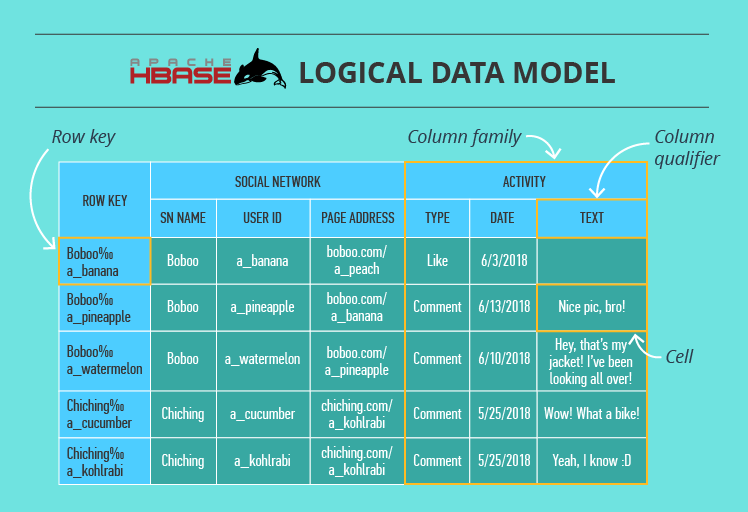
\includegraphics[scale=0.45]{img/wide-column-hbase.png}
	\captionsource{Schéma du principe de stockage de cassandra}{http://www.alliedc.com/apache-cassandra-database-4-problems-that-cassandra-developers-administrators-face/}
	\label{wide-column-hbase}
\end{figure}

\subsubsection{Cassandra}
\label{cassandra}

Consistent, meilleur en écriture, solution native

La figure {\ref{wide-column-cassandra}} représente un exemple de la manière dont sont stocker les données dans Cassandra.

\begin{figure}[!h]
	\centering 
	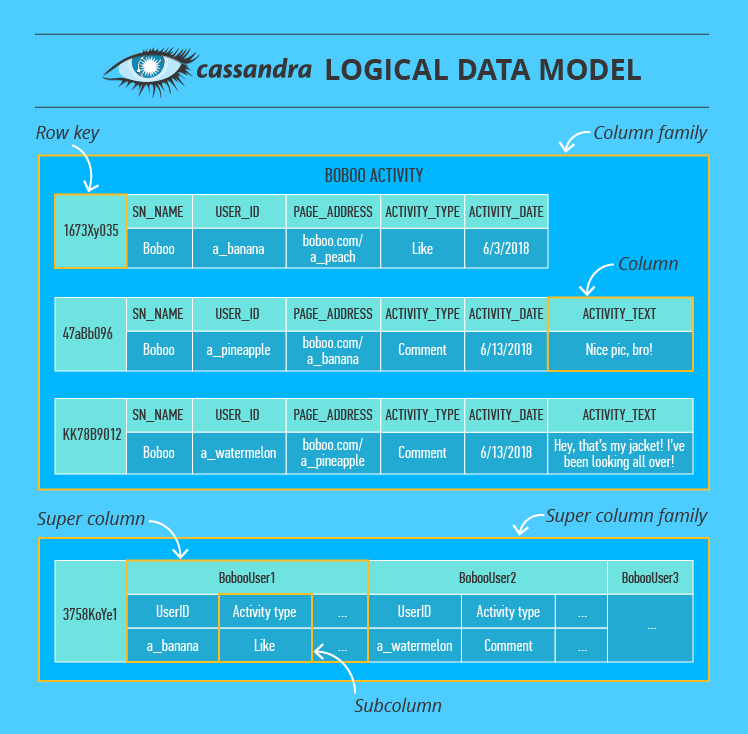
\includegraphics[scale=0.45]{img/wide-column-cassandra.png}
	\captionsource{Schéma du principe de stockage de cassandra}{http://www.alliedc.com/apache-cassandra-database-4-problems-that-cassandra-developers-administrators-face/}
	\label{wide-column-cassandra}
\end{figure}

\subsection{Système de fichiers}

\subsubsection{Hadoop HDFS}
\label{hdfs}

\section{Requêtage des données}

Afin de permettre l'analyse et la visualisation des données, il est nécessaire de requêter les données stockées dans des bases de données. Pour cela il y a deux possibilités. La première solution est d'utiliser les outils de requêtage fournit par les bases de données, et la seconde est d'utiliser des librairies externes permettant d'uniformiser le requêtage entre les différentes bases de données.

Aujourd'hui, les solutions de stockage propose des solutions de requêtage qui essaient d'être le plus simple possible tout en conservant des performances suffisante. L'utilisation de librairie externe est surtout utile si vous ne souhaitez pas apprendre les requêtes pour chacune des bases de données que vous utilisez. Étant donnée que ces solutions de requêtage ne sont pas primordiale et que ce mémoire traite déjà de beaucoup de technologies, nous n'allons pas nous intéresser à ces solutions. je voulais juste préciser que de telles solutions existait, et je vous laisse vous renseigner si cela vous intéresse.

\section{Visualisation et Analyse des données}

\subsection{Kibana}
\label{kibana}

Comme Banana mais pour ES.

\subsection{Banana}
\label{banana}

Comme Kibana mais pour Solr

\subsection{Grafana}

Se plug partout. Spécialisé dans le monitoring.

\subsection{Tableau}

\subsection{Click}

\section{Orchestration}

Les solutions Big Data ont besoin d'un moyen de programmer l'exécution de certaines tâches, par exemple l'exécution de l'ingestion des données d'une source de données ou bien la création d'un rapport sur un outil d'analyse. C'est pour cela que l'on utilise un orchestrateur.

\subsection{Apache Oozie}

Apache Oozie est une solution open source sous la licence Apache 2 écrit en Java et développé par Apache.

Apache Oozie est conçu pour fonctionner avec les outils Hadoop (MapReduce et HDFS par exemple), mais il dispose aussi de fonctionnalités pour programmer l'exécution de script Shell ou Java.

Oozie permet de définir une chaîne d'actions à effectuer à un moment précis, il permet aussi d'effectuer une autre action si jamais une des tâches de la chaîne échoue. Afin de paramétrer cette chaîne d'action, Oozie propose aux utilisateurs une interface graphique pour faciliter sa configuration.

Permet de faire des chaînes d'actions.
Interface graphique.

\subsection{Cron}

Une solution beaucoup plus basique et qui existe depuis longtemps, est l'utilisation de la cron tab sous Linux. Cette solution propose uniquement de lancer une tâche tout les x temps, mais avec l'utilisation des messages broker, il n'est pas forcément nécessaire de lancer une suite de tâche. En effet, si les messages brokers permettent de déclencher des évènements afin de récupérer les données, les envoyer au logiciel de traitement de données puis les stocker dans la base de données sélectionnée, la seule tâche restante est la génération d'un rapport. L'utilisation de la cron tab est suffisante pour ce genre de tâche et ne nécessite aucune installation, car elle est installée avec Linux.

\subsubsection{Conclusion}

Nous pouvons constater que la partie orchestration ne nécessite pas d'avoir une solution très avancée, même des solution basiques suffisent. Mais si l'on veut pouvoir facilement configurer l'exécution de nos tâches des solutions graphique sont tout de même à notre disposition.
